% Slide Template
% Omslut slides med \begin{frame} og \end{frame}
% Standard LaTeX syntaks benyttes (itemize, tabular osv)
% Husk at tilføje eventuelle packages i headeren

\begin{frame}
\frametitle{Statistik}
\framesubtitle{Hvordan bliver lommepenge brugt?} % VALGFRI - kan fjernes

%\hfill
%	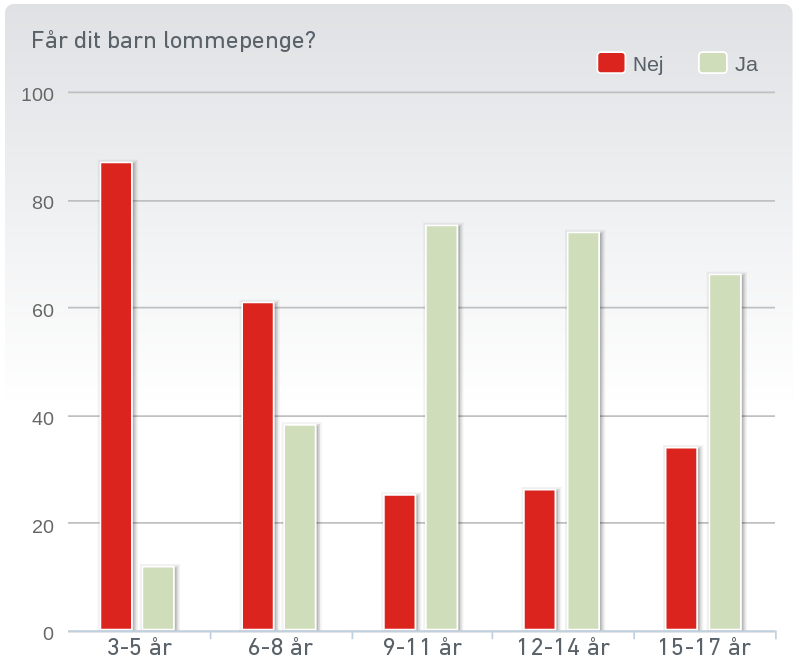
\includegraphics[width=0.6\textwidth]{../../Billeder/FaarBarnLommepenge.png}
    \begin{multicols}{2}
  \noindent
	 	 \begin{itemize}
        	\item{Syv ud af ti skal udføre pligter for pengene.}
        		\begin{itemize}
        			\item Heraf får halvdelen mindre, hvis opgaverne ikke bliver udført.
        		\end{itemize}
        	\item{Seks ud af ti kan tjene ekstra penge.}
        	\item{Alligevel mange der ender med gæld.}
        	\item{Her er der gode muligheder for at lære børn endnu mere om økonomi.}
    	\end{itemize}
 	\columnbreak
 	    \noindent
 	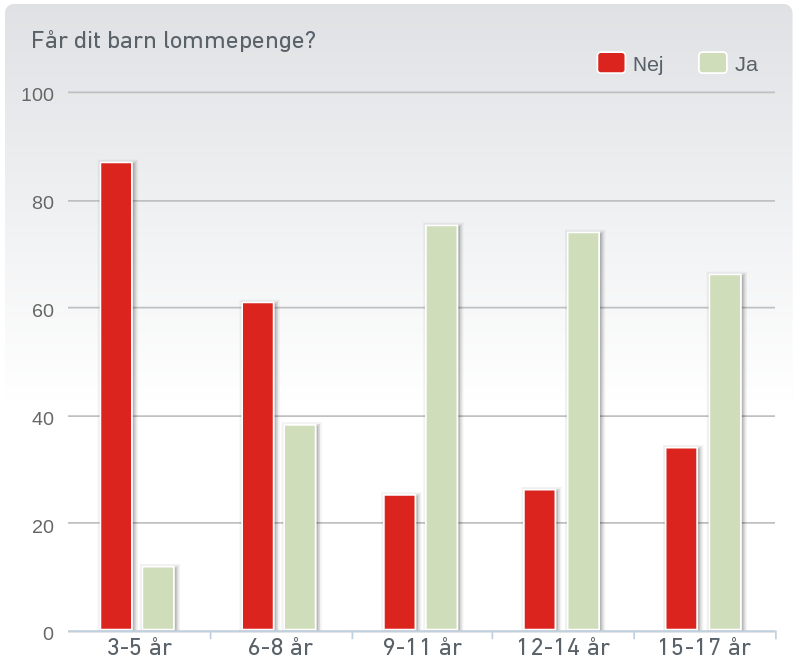
\includegraphics[width=0.55\textwidth]{../../Billeder/FaarBarnLommepenge.png}
    \end{multicols}
\end{frame}
    
%\begin{frame} ....